\documentclass[manuscript]{acmart}
\usepackage[utf8]{inputenc}
% for figures
\usepackage{tikz}
% for subfigures
\usepackage{subcaption}

\begin{document}
\title{Brief Announcement: Byzantine Eventual Consistency}
\author{Martin Kleppmann}
\email{mk428@cst.cam.ac.uk}
\orcid{0000-0001-7252-6958}
\affiliation{%
  \institution{University of Cambridge}
  \streetaddress{15 JJ Thomson Avenue}
  \city{Cambridge}
  \postcode{CB3 0FD}
  \country{UK}
}

\author{Heidi Howard}
\email{hh360@cst.cam.ac.uk}
\orcid{0000-0001-5256-7664}
\affiliation{%
  \institution{University of Cambridge}
  \streetaddress{15 JJ Thomson Avenue}
  \city{Cambridge}
  \postcode{CB3 0FD}
  \country{UK}
}

\begin{abstract}
    TODO
\end{abstract}
\maketitle

\section{Introduction}

Byzantine agreement assumes that at most $f$ of $n$ processes are byzantine-faulty.
It is well established that without synchrony, byzantine agreement is impossible if $n\leq3f$~\cite{Lamport:1982,Dwork:1988,Fischer:1985}.
If more than $f$ processes are faulty, neither safety nor liveness can be guaranteed.
This is a problem because the $f$-faulty assumption is not always a realistic threat model.
Byzantine failures are not necessarily independent, if an adversary can compromise one of the processes (e.g. due to a software vulnerability), it is likely that they can compromise a majority of processes, since they are likely to all be running the same software. 
% same is true for software bugs
This issue was acknowledged in the pBFT paper, where it stated that: `... each node should run different implementations of the service code and operating system...'~\cite{Castro:1999}. 
Clearly, this is infeasible for any system with more than a few processes and thus is seldom true in practice today.
Moreover, in some systems, the adversary may be able to spawn a large number of processes, and thus create a majority of Byzantine-faulty processes (this is known as a Sybil attack~\cite{Douceur:2002jr}).

This raises the question: if consensus cannot be achieved in the face of arbitrary numbers of Byzantine-faulty processes, what consistency model can we achieve?

\emph{Strong Eventual Consistency} (SEC)~\cite{Shapiro:2011un} is a consistency model in which replicas eventually converge towards the same state as they communicate.
SEC is defined in a non-Byzantine model, and we define \emph{Byzantine Eventual Consistency} (BEC) is a generalisation of SEC to a Byzantine model.
BEC can be achieved regardless of the number of Byzantine-faulty processes.

Define the safety and liveness properties of BEC, in analogy to the correctness properties for consensus.
The idea is: whenever any two correct processes communicate, they converge towards the same state, regardless of what communication with Byzantine-faulty processes may have taken place.

We can implement BEC as follows. First define the state of a replica to be a deterministic function of the set of updates that has occurred (where the set has no order).
Thus, any two replicas that have seen the same set of updates must also be in the same state, regardless of the order in which the replicas received the updates. This is exactly what a CRDT does.
We can prove that CRDTs achieve SEC in a non-Byzantine model.

For example, say we want the state to be a totally ordered log of values.
Each update adds a value to the log; assume that each update contains a value, a timestamp, and the unique ID of the process that produced the update.
We can define the log to be simply the set of values appearing in the updates, sorted by timestamp, breaking ties based on ordering of process IDs.

Thus, achieving BEC boils down to ensuring that whenever two correct processes communicate, they end up with the same set of updates.
The simplest way of achieving this is with the trivial reconciliation algorithm: each replica stores the set of all updates it has seen; whenever two replicas communicate, they send each other their entire sets of updates; on receiving such a set, a replica computes the union of existing and incoming updates, and stores that set.

That reconciliation is obviously inefficient. To avoid redundant network traffic, we want replicas to send each other only those updates that the other replica is missing.
How do we do this?
Some systems do this using vector clocks, but vector clocks don't work well in a Byzantine system, because a Byzantine-faulty node could send different updates to different recipient processes under the same vector timestamp, causing two replicas to have the same vector timestamps, but different sets of updates, causing them to become inconsistent.

To improve the reconciliation protocol, we first add hash chaining.
That is: whenever a replica produces an update, it includes in the update the hashes of all existing updates whose hashes have not already been included in another update (in the replica's local set of updates).
The result is a DAG of updates referencing other updates, much like a Git commit history.
We use a cryptographic (collision-free) hash function so that it is not feasible for an adversary to generate two different updates with the same hash.

The updated reconciliation protocol now looks like this: when two replicas connect, they first send each other the hashes of all updates in their local set that are not referenced by another update (the ``heads'' in Git terminology).
On receiving a hash, if the recipient knows an update with that hash, it sends back all updates that reference the received hash, directly or indirectly (since it knows that the other side doesn't have these updates).
If the recipient does not have an update with that hash, it sends back its heads.
In this case, the protocol will have to run for several rounds, gradually working from the heads backwards until the replicas find an update that they have in common.

If the communication is between a correct and a Byzantine-faulty replica, the faulty replica can obviously add updates to the set or omit updates from those sent to the correct replica.
But the faulty replica cannot corrupt the correct replica's state in a way that would prevent the correct replica from later synchronising its set of updates with another correct replica.

To reduce the number of rounds of communication in this protocol, perhaps the replicas can send Bloom filters to each other, summarising the set of updates they know about.
Need to think carefully about how Bloom filter false positives are handled, though. TODO

\section{Properties}

A frequent use for consensus algorithms is to generate an append-only log of values that can be used for state machine replication.
When using Byzantine agreement to generate this log, we require that the following properties hold:

\begin{description}
\item[Validity:] Any value decided by a correct process must have been proposed by one of the processes.
\item[Agreement:] When any two correct processes decide a value for a certain position in the log, those decided values are the same.
\item[Liveness:] For any value proposed, correct processes will eventually decide that value for some position in the log.
\end{description}

Validity must hold regardless of the number of fault or the synchrony model.
Agreement must hold provided at most $f$ processes are byzantine-faulty but regardless of the number of crash-faults and synchrony. 
Liveness must hold provided at most $f$ processes are byzantine-faulty and assuming partial synchrony~\cite{Dwork:1988}.

We can define a similar set of properties for Byzantine eventual consistency.
These properties are weaker, but they hold without making any assumptions about the number of faulty processes:

\begin{description}
\item[Validity:] Any value contained in the log of a correct process must have been proposed by one of the processes.
\item[Convergence:] When any two correct processes finish communicating, their logs are the same.
\item[Ordering:] If the log of two correct processes both contain values A and B, then A and B appear in the same order in both logs.
\item[Liveness:] Assuming that any two correct processes will eventually finish communicating, a value proposed by one process will eventually be contained in the log of all correct processes.
\end{description}

\section{Reconciliation Algorithm}

Assume every process locally maintains a monotonically growing set of updates $\mathcal{U}$.
(We discuss in Section~\ref{sec:optimisations} how to prevent unbounded storage growth.)
When two processes $p$ and $q$ communicate, and each process initially has updates $\mathcal{U}_p$ and $\mathcal{U}_q$ respectively, the purpose of a reconciliation algorithm is that both processes converge to the same set $\mathcal{U}_q \cup \mathcal{U}_q$.

The simplest reconciliation algorithm is for $p$ to send $\mathcal{U}_p$ to $q$, and vice versa, and for both processes to compute the union of the received set of updates with its local set.
This algorithm works, but if there is a lot of overlap between the two sets, it results in a large amount of data being unnecessarily transmitted.
Thus, in this section we introduce a more efficient algorithm.

Let the set of updates $\mathcal{U} \subseteq \mathit{Timestamp} \times \mathit{Value} \times \mathcal{P}(\mathit{Hash})$ be a set of triples $(t, v, \mathit{hs})$, where $t$ is any kind of totally ordered timestamp (e.g. a Lamport timestamp~\cite{Lamport:1978}), $v$ is any value, and $\mathit{hs}$ is a set of hashes produced by a hash function $H(\cdot)$.
We assume that $H$ returns a short, fixed-length bit string (e.g.\ 256 bits in the case of SHA-256), and that $H$ is collision-resistant (i.e.\ it is computationally infeasible to find distinct $x$ and $y$ such that $H(x) = H(y)$).

Whenever a process generates an update $(t, v, \mathit{hs})$, $\mathit{hs}$ is defined to be the set of hashes of all existing updates in $\mathcal{U}$ whose hashes have not already been included in another update:
\[
\mathit{hs}_\mathsf{new} = \{H(u) \mid u \in \mathcal{U} \wedge \nexists (t, v, \mathit{hs}) \in \mathcal{U}.\; H(u) \in \mathit{hs}\}
\]
The result is a directed acyclic graph (DAG) of updates referencing other updates via their hashes, like a Git commit history.
We can assume that the graph is acyclic because the presence of a cycle would imply knowledge of a collision.

We define the set of successors $\mathrm{succ}^1(u)$ of an update $u$ to be the set of updates that reference $H(u)$; we define $\mathrm{succ}^2(u)$ to be the successors of the successors of $u$, and so on, and define $\mathrm{succ}^*(u)$ to be the transitive closure:
\[
\mathrm{succ}^i(u) =
\begin{cases}
\{(t, v, \mathit{hs}) \in \mathcal{U} \mid H(u) \in \mathit{hs}\} & \text{ for } i=1 \\
\bigcup_{u' \in \mathrm{succ}^1(u)} \mathrm{succ}^{i-1}(u') & \text{ for } i>1
\end{cases}
\quad\quad\quad\quad
\mathrm{succ}^*(u) = \bigcup_{i \ge 1} \mathrm{succ}^i(u)
\]

\begin{figure}
    \centering
    \begin{subfigure}[t]{0.3\textwidth}
    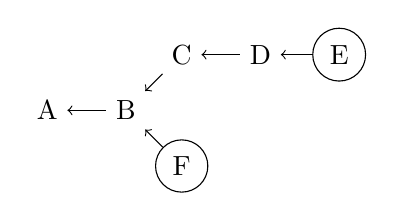
\begin{tikzpicture}

% nodes
\node (a) {A};
\node (b) [right of=a] {B};
\node (c) [above right of=b] {C};
\node (d) [right of=c] {D};
\node[circle,draw] (e) [right of=d] {E};
\node[circle,draw] (f) [below right of=b] {F};

% arrows
\draw[<-] (a) -- (b);
\draw[<-] (b) -- (c);
\draw[<-] (c) -- (d);
\draw[<-] (d) -- (e);
\draw[<-] (b) -- (f);
\end{tikzpicture}
    \caption{$p_1$ before reconciliation}
    \end{subfigure}
    \begin{subfigure}[t]{0.3\textwidth}
    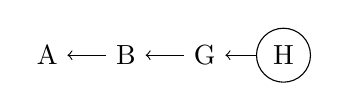
\begin{tikzpicture}

% nodes
\node (a) {A};
\node (b) [right of=a] {B};
\node (g) [right of=b] {G};
\node (h)[circle,draw] [right of=g] {H};

% arrows
\draw[<-] (a) -- (b);
\draw[<-] (b) -- (g);
\draw[<-] (g) -- (h);
\end{tikzpicture}
    \caption{$p_2$ before reconciliation}
    \end{subfigure}
    \begin{subfigure}[t]{0.3\textwidth}
    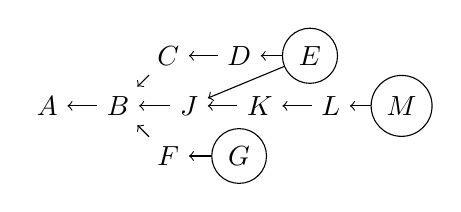
\begin{tikzpicture}[node distance=0.9cm]

% nodes
\node (a) {$A$};
\node (b) [right of=a] {$B$};
\node (c) [above right of=b] {$C$};
\node (d) [right of=c] {$D$};
\node (e) [right of=d,draw,circle] {$E$};
\node (j) [right of=b] {$J$};
\node (k) [right of=j] {$K$};
\node (l) [right of=k] {$L$};
\node (m) [right of=l,draw,circle] {$M$};
\node (f) [below right of=b] {$F$};
\node (g) [right of=f,draw,circle] {$G$};

% arrows
\draw[<-] (a) -- (b);
\draw[<-] (b) -- (c);
\draw[<-] (c) -- (d);
\draw[<-] (d) -- (e);
\draw[<-] (b) -- (j);
\draw[<-] (j) -- (e);
\draw[<-] (j) -- (k);
\draw[<-] (k) -- (l);
\draw[<-] (l) -- (m);
\draw[<-] (b) -- (f);
\draw[<-] (f) -- (g);
\end{tikzpicture}
    \caption{$p_1$ and $p_2$ after reconciliation}
    \end{subfigure}
    \caption{Caption}
    \label{fig:my_label}
\end{figure}

\begin{figure}
    \centering
    \vspace{0.5cm}
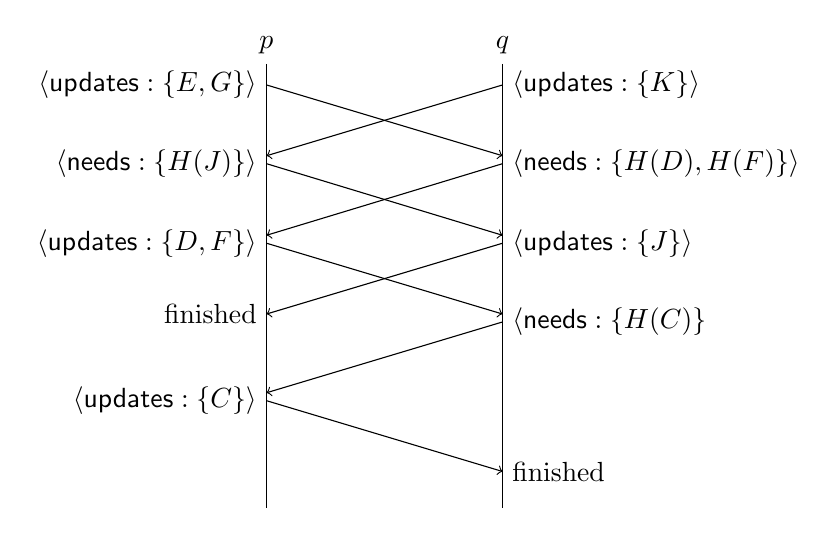
\begin{tikzpicture}
\def\width{3cm}
\def\latency{1cm}
\def\spacing{0.1cm}
\def\length{6cm}
\def\startdelay{0.5cm}

% Timelimes
\node (p1-start) at (0,0) {$p$};
\node (p2-start) at (\width,0) {$q$};
\node (p1-end) at (0,-\length) {};
\node (p2-end) at (\width,-\length) {};
\draw (p1-start) -- (p1-end);
\draw (p2-start) -- (p2-end);

% Messages
\draw[->] (0,-\startdelay) node[left] {$\langle\mathsf{updates}: \{E,G\}\rangle$} -- (\width,\spacing-\startdelay-\latency);
\draw[->] (\width,-\startdelay) node[right] {$\langle\mathsf{updates}: \{K\}\rangle$} -- (0,\spacing-\startdelay-\latency);

\draw[->] (\width, -\startdelay-\latency) node[right] {$\langle\mathsf{needs}: \{H(D), H(F)\}\rangle$} -- (0,\spacing-\startdelay-2.0\latency);
\draw[->] (0, -\startdelay-\latency) node[left] {$\langle\mathsf{needs}: \{H(J)\}\rangle$} -- (\width,\spacing-\startdelay-2.0\latency);

\draw[->] (0, -\startdelay-2.0\latency) node[left] {$\langle\mathsf{updates}: \{D, F\}\rangle$} -- (\width,\spacing-\startdelay-3.0\latency);
\draw[->] (\width, -\startdelay-2.0\latency) node[right] {$\langle\mathsf{updates}: \{J\}\rangle$} -- (0,\spacing-\startdelay-3.0\latency) node[left] {finished};

\draw[->] (\width, -\startdelay-3.0\latency) node[right] {$\langle\mathsf{needs}: \{H(C)\}$} -- (0,\spacing-\startdelay-4.0\latency);

\draw[->] (0, -\startdelay-4.0\latency) node[left] {$\langle\mathsf{updates}: \{C\}\rangle$} -- (\width,\spacing-\startdelay-5.0\latency) node[right] {finished};

\end{tikzpicture}
    \caption{Caption}
    \label{fig:my_label}
\end{figure}

\subsection{Optimisations}\label{sec:optimisations}

\section{Related Work}

Byzantine agreement has been subject of extensive research since the early 80s~\cite{Lamport:1982} and has seen a recent renewal of interest due to its application in blockchains~\cite{Bano:2019}.
Most algorithms including PBFT~\cite{Castro:1999}, HQ~\cite{Cowling:2006}, Zyzzyva~\cite{Kotla:2007}, Aliph~\cite{Aublin:2015} and HotStuff~\cite{Yin:2019} assume that $n=3f+1$, whereas Q/U~\cite{Abd:2005} and FaB~\cite{Martin:2006} require that $n=5f+1$.
Some algorithm take a different approach, for example, Upright~\cite{Clement:2009} separates the number of crash failures ($u$) and byzantine failures ($r$) and assumes $n=2u+r+1$.


% Roy Friedman and Roni Licher. Hardening Cassandra Against Byzantine Failures.
% https://arxiv.org/pdf/1610.02885.pdf

% Ali Shoker et al. As Secure as Possible Eventual Consistency: Work in Progress (PaPoC 2017)
% https://dl.acm.org/doi/10.1145/3064889.3064895

% Wenbing Zhao and Mamdouh Babi. Byzantine fault tolerant collaborative editing.
% https://pdfs.semanticscholar.org/587b/c024d5e877608c79f484112666489d90f041.pdf

% Git fetch negotiation algorithm, How does this compare to git fetch negotiation algorithms, default and skipping?  
% https://stackoverflow.com/questions/40484929/will-a-git-pull-develop-fetch-all-the-commits-reacheable-from-develop
% https://git-scm.com/docs/git-config#Documentation/git-config.txt-fetchnegotiationAlgorithm

% Comparison to Julien Quintard work on byzantine file systems https://www.repository.cam.ac.uk/bitstream/handle/1810/243442/thesis.pdf?sequence=1&isAllowed=y
% https://infinit.sh

% Comparison to irmin
% https://mirage.github.io/irmin/irmin/Irmin/index.html#syncing-with-a-remote
% https://github.com/mirage/irmin/blob/master/src/irmin/sync_ext.ml#L86-L123

% Comparision to byzantine quorums
% http://www.cs.cornell.edu/courses/cs5414/2017fa/papers/bquorum-dc.pdf

% Comparision to byz chain replication
% https://link.springer.com/chapter/10.1007/978-3-642-35476-2_24

\begin{acks}
Martin Kleppmann is supported by a Leverhulme Trust Early Career Fellowship, and by the Isaac Newton Trust.
\end{acks}

\bibliographystyle{ACM-Reference-Format}
\bibliography{references}
\end{document}
